On dispose d'une boîte opaque contenant 7 boules blanches identiques et indiscernables au toucher. Les boules sont numérotées de 1 à 7.

\begin{enumerate}
	\item On s'intéresse aux boules dont le numéro est un nombre premier.
	\begin{enumerate}
		\item Citer les numéros de boules correspondant à des nombres premiers.
		\item Vérifier que la probabilité d'obtenir une boule dont le numéro est un nombre premier est de $\dfrac{4}{7}$.
	\end{enumerate}
	\item On réalise l'expérience suivante : \og On tire au sort une boule de la boîte, on note le numéro qu'elle porte puis on remet la boule dans la boîte \fg.
	
	On répète cette expérience 100 fois. Le diagramme en bâtons ci-après représente la fréquence d'apparition de chacun des numéros.

\begin{center}
		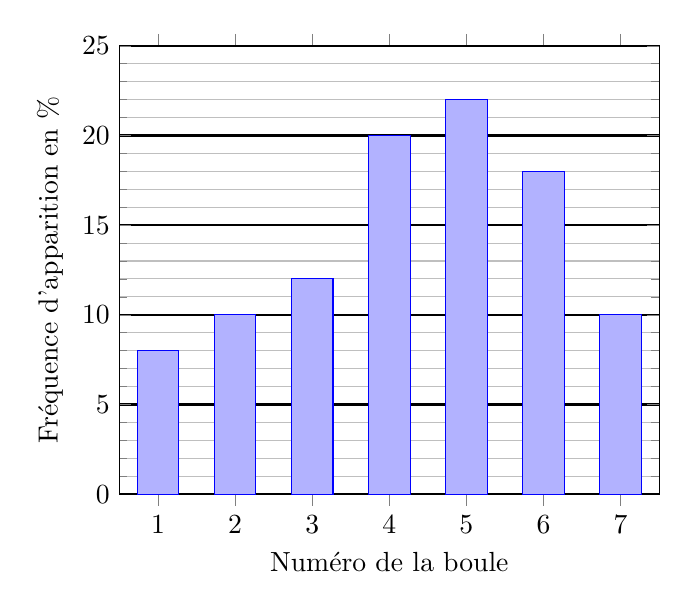
\begin{tikzpicture}
			\begin{axis}[
				title={},
				xlabel={Numéro de la boule},
				ylabel={Fréquence d'apparition en \%},
				xmin=0.5, xmax=7.5,
				ymin=0, ymax=25,
				ytick={0,5,10,15,20,25},
				ymajorgrids=true,                  
				major grid style={black, thick},   
				yminorgrids=true,                  
				minor y tick num=4,                
				minor grid style={lightgray},      
				ybar,
				bar width=15pt
			]
			\addplot coordinates {(1,8) (2,10) (3,12) (4,20) (5,22) (6,18) (7,10)};
			\end{axis}
		\end{tikzpicture}
	\end{center}

	\begin{enumerate}
		\item En utilisant ce diagramme en bâtons, déterminer la fréquence d'apparition de la boule qui porte le numéro 2.
		\item Vérifier que la somme des fréquences d'apparition des boules dont le numéro est un nombre premier est égale à $54\,\%$.
	\end{enumerate}
	\item D'après les questions précédentes, on dispose des informations suivantes :
	\begin{itemize}
		\item la probabilité d'obtenir un nombre premier est $\dfrac{4}{7}$ ;
		\item la fréquence d'apparition d'un nombre premier est de $54\,\%$.
	\end{itemize}
	\begin{enumerate}
		\item Montrer que $\dfrac{4}{7}$ n'est pas égal à $54\,\%$.
		\item Expliquer pour quelle raison la probabilité calculée et la fréquence d'apparition mesurée ne donnent pas la même valeur.
	\end{enumerate}
\end{enumerate}

\needspace{10\baselineskip}
